\tikzset{every picture/.style={line width=0.75pt}} %set default line width to 0.75pt        

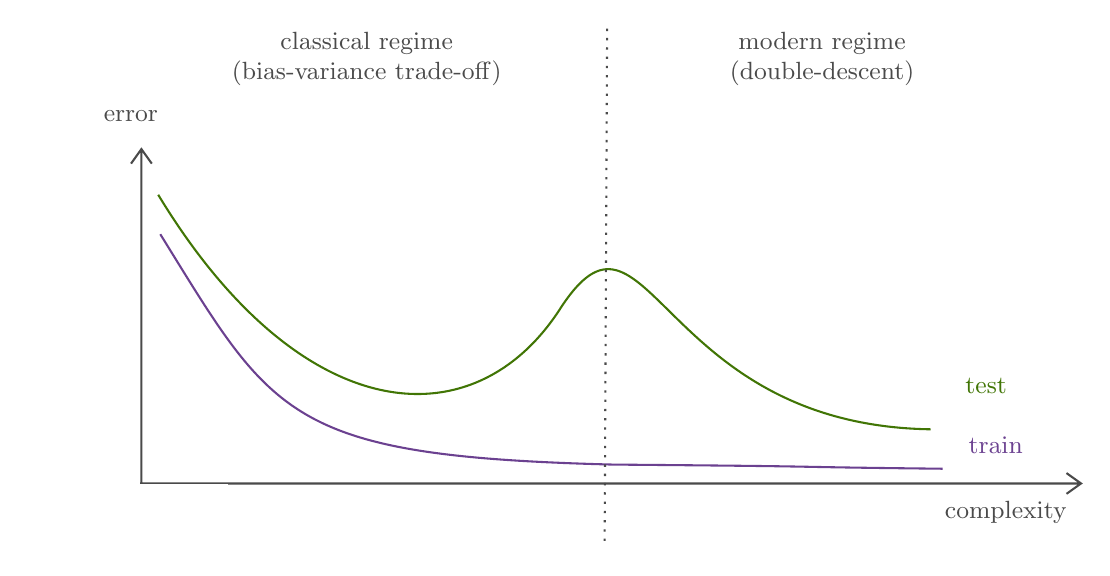
\begin{tikzpicture}[x=0.75pt,y=0.75pt,yscale=-1,xscale=1]
%uncomment if require: \path (0,296); %set diagram left start at 0, and has height of 296

%Shape: Axis 2D [id:dp20000513897555317] 
\draw [color={rgb, 255:red, 74; green, 74; blue, 74 }  ,draw opacity=1 ] (28.5,245.1) -- (531.5,245.1)(78.8,84) -- (78.8,263) (524.5,240.1) -- (531.5,245.1) -- (524.5,250.1) (73.8,91) -- (78.8,84) -- (83.8,91)  ;
%Curve Lines [id:da4390231353399854] 
\draw [color={rgb, 255:red, 65; green, 117; blue, 5 }  ,draw opacity=1 ]   (86.89,106) .. controls (154.77,218) and (238.5,226) .. (280.5,161) .. controls (322.5,96) and (326.88,217) .. (458.99,219) ;
%Curve Lines [id:da6461413451688074] 
\draw [color={rgb, 255:red, 107; green, 65; blue, 144 }  ,draw opacity=1 ]   (87.89,125) .. controls (139,207.46) and (147.54,229.33) .. (278.05,235.05) .. controls (286.82,235.44) and (296.14,235.75) .. (306.06,236) .. controls (426.05,237) and (375.15,237) .. (464.84,238) ;
%Shape: Rectangle [id:dp3984656798297582] 
\draw  [color={rgb, 255:red, 255; green, 255; blue, 255 }  ,draw opacity=1 ][fill={rgb, 255:red, 255; green, 255; blue, 255 }  ,fill opacity=1 ] (24.5,216) -- (77.59,216) -- (77.59,256) -- (24.5,256) -- cycle ;
%Shape: Rectangle [id:dp9250237166695404] 
\draw  [color={rgb, 255:red, 255; green, 255; blue, 255 }  ,draw opacity=1 ][fill={rgb, 255:red, 255; green, 255; blue, 255 }  ,fill opacity=1 ] (35.17,246) -- (120.01,246) -- (120.01,266) -- (35.17,266) -- cycle ;
%Straight Lines [id:da006727548782663129] 
\draw [color={rgb, 255:red, 74; green, 74; blue, 74 }  ,draw opacity=1 ] [dash pattern={on 0.84pt off 2.51pt}]  (303.18,26) -- (301.97,275.5) ;

% Text Node
\draw (464.43,252) node [anchor=north west][inner sep=0.75pt]  [font=\small,color={rgb, 255:red, 74; green, 74; blue, 74 }  ,opacity=1 ] [align=left] {complexity};
% Text Node
\draw (59.16,64) node [anchor=north west][inner sep=0.75pt]  [font=\small,color={rgb, 255:red, 74; green, 74; blue, 74 }  ,opacity=1 ] [align=left] {error};
% Text Node
\draw (475.9,221) node [anchor=north west][inner sep=0.75pt]  [font=\small,color={rgb, 255:red, 107; green, 65; blue, 144 }  ,opacity=1 ] [align=left] {train };
% Text Node
\draw (457.88,193) node [anchor=north west][inner sep=0.75pt]  [font=\small,color={rgb, 255:red, 65; green, 117; blue, 5 }  ,opacity=1 ] [align=left] {\quad \ test};
% Text Node
\draw (103.43,26) node [anchor=north west][inner sep=0.75pt]  [font=\small,color={rgb, 255:red, 74; green, 74; blue, 74 }  ,opacity=1 ] [align=left] {\begin{minipage}[lt]{123.62pt}\setlength\topsep{0pt}
\begin{center}
classical regime\\(bias-variance trade-off)
\end{center}

\end{minipage}};
% Text Node
\draw (349.13,26) node [anchor=north west][inner sep=0.75pt]  [font=\small,color={rgb, 255:red, 74; green, 74; blue, 74 }  ,opacity=1 ] [align=left] {\begin{minipage}[lt]{84.16pt}\setlength\topsep{0pt}
\begin{center}
modern regime\\(double-descent)
\end{center}

\end{minipage}};


\end{tikzpicture}